\section{Temporary Interruptions}
In this section, we discuss how VCAs respond to controlled interruptions during the call.  

\begin{figure}[]
    \centering
    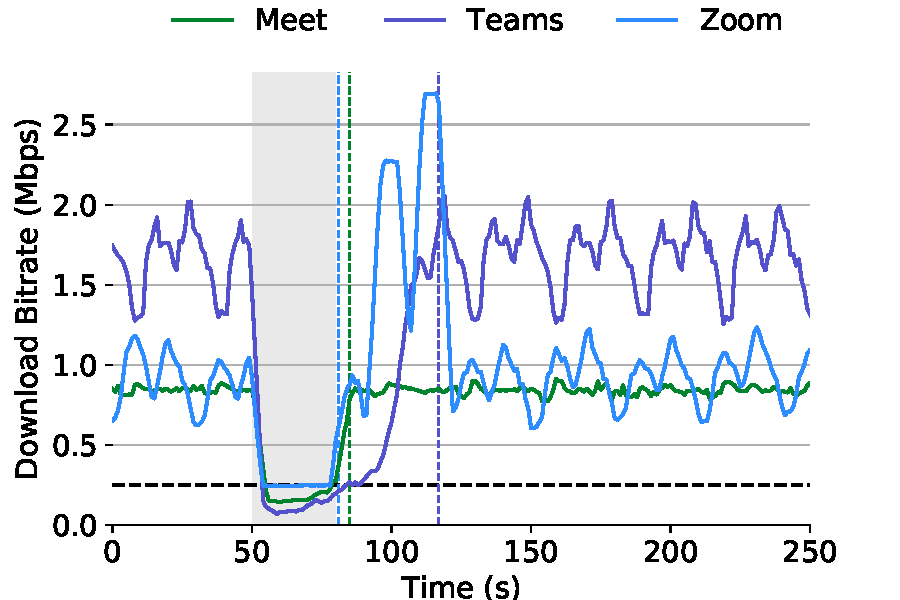
\includegraphics[width=0.45\textwidth,keepaspectratio]{interrupt/Interrupt-dnld.pdf}
    \caption{Downlink Throughput over Time. The gray region indicates when the downlink bandwidth was lowered to 0.25Mbps}
    \label{fig:interrupt-dnld}
\end{figure}
\begin{figure}[]
    \centering
    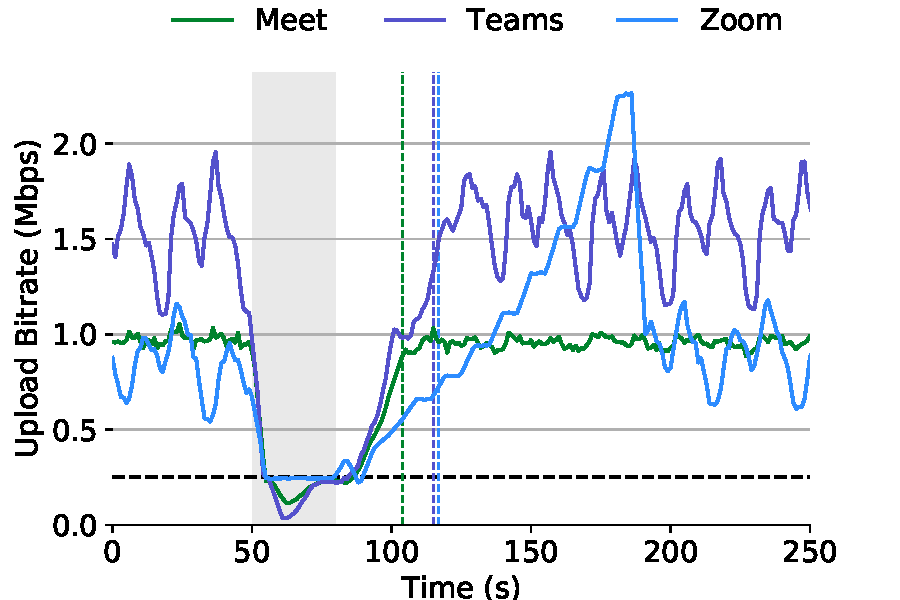
\includegraphics[width=0.45\textwidth,keepaspectratio]{../figures/interrupt/Interrupt-upld.pdf}
    \caption{Loss and QoS metrics zoom}
    \label{fig:Interrupt_upld}
\end{figure}


\begin{figure*}[ht]
\begin{subfigure}[t]{.5\textwidth}
  \centering
    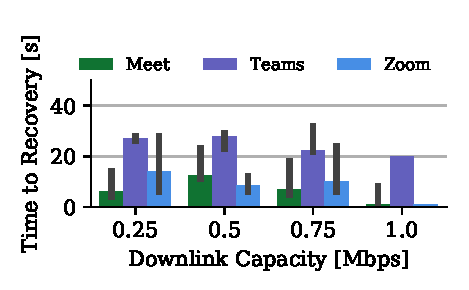
\includegraphics[width=1\textwidth,keepaspectratio]{../figures/interrupt/TTR-dnld.pdf}
    \captionsetup{width=.9\linewidth}
    \caption{Meet and Zoom recover quickly from downlink interruptions, while Teams takes consistently longer.}
    \label{fig:TTR_dnld}
\end{subfigure}
\begin{subfigure}[t]{.5\textwidth}
  \centering
    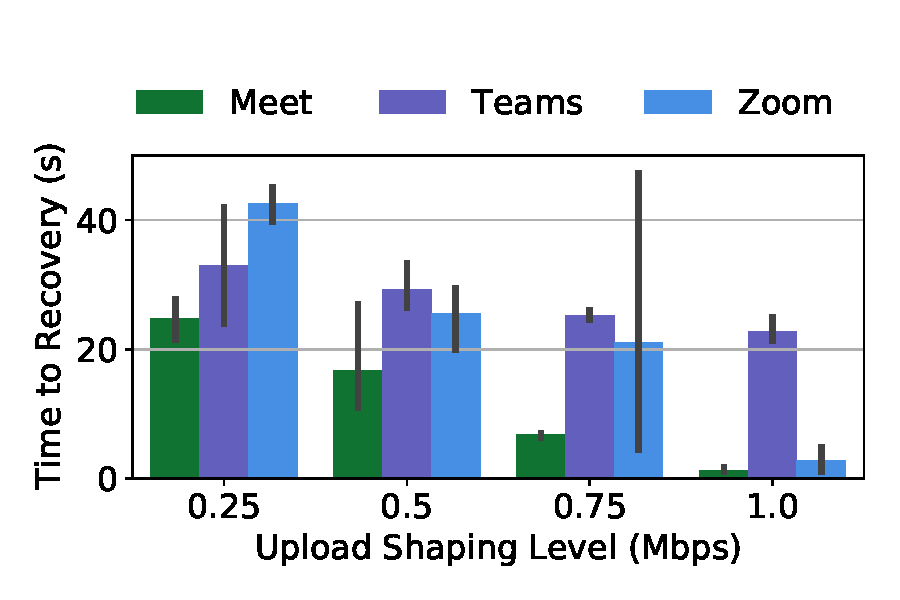
\includegraphics[width=1\textwidth,keepaspectratio]{../figures/interrupt/TTR-upld.pdf}
    \captionsetup{width=.9\linewidth}
    \caption{Time to recovery increases with the severity of the uplink interruption}
    \label{fig:TTR_upld}
\end{subfigure}
\caption{The time to recovery is the time needed to return to the nominal rate following a drop in bandwidth}
\label{fig:TTR}
\end{figure*}



\noindent \textbf{Methodology}:
Using the same setup as Figure \ref{fig:static_setup}, a VCA call is initiated between two clients, C1 and C2, both of which sit behind unconstrained links. Once the VCA reaches its nominal consumption, we reduce the available bandwidth between C1 and the router for 30 seconds, before reverting back to an unconstrained link.  

We introduce the metric \textit{time to recovery} (TTR) in order to compare how the different VCAs respond to the interruption. We define TTR as the time 
between when the interruption ends and when the 5 second rolling median bitrate reaches the default bitrate. In other words, how long it takes the VCA performance to return to normal following the interruption.

\noindent \textbf{Discussion}: 
The VCAs differ greatly in their response to interruptions, with some recovering much faster than others. Focusing first on download shaping, it is clear that Teams recovers much slower than Meet and Zoom, always taking at least 20 seconds longer to return to the nominal rate, regardless of the magnitude of the interruption. This can be explained by the way each VCA sends video. 

In all three VCAs, C1 and C2 communicate through an intermediary server. Meet uses an encoding technique called \textit{simulcast}, where the client encodes two versions . The server then sends the appropriate version based on the perceived downlink capacity at the receiver. This way, a sender transmitting on an unconstrained link does not have to adjust its sending and can rely on the server to send the appropriate version. The server can then quickly switch between which version to send to the receiver based on the feedback it receives. This quick recovery is clearly illustrated in \ref{fig:interrupt-dnld}, in which Meet returns to its nominal rate in under 10 seconds, depending on the severity of the interruption.

Similarly, Zoom uses \textit{multi-bitrate encoding} when transmitting video. Instead of sending several versions of varying quality, Zoom sends many "layers" that, when superimposed, produce a high quality video. 

While the intermediary server for Zoom and Meet does congestion control, it only acts as a relay for Teams. So during a Teams call, C2 will recognize C1 has limited downlink capacity and adjust its behavior, sending at only the bitrate it knows C1 can handle. Once the C1 has more available bandwidth, however, C2 must first probe the connection before returning to its nominal sending rate. As a result, Teams recovers much slower than Zoom and Meet.

Turning now to upload shaping, we observe longer recovery times for all three VCAs. There is a clear trend that the more severe the upload shaping, the longer the VCAs need to recover. While Meet and Teams have a fairly direct recovery trend, Figure \ref{fig:Interrupt_upld} shows how Zoom slowly increases the sending bitrate, going well above the nominal rate, before finally dropping back to steady state. 

The differences in recovery time can be partial explained by the differences in each application's nominal rate, in which Teams sends and receives at a much higher rate than Meet and Zoom. 







